% Compile with XeLaTeX (Overleaf: Menu -> Compiler -> XeLaTeX) or `tectonic main.tex`.
\documentclass[11pt,a4paper]{article}

\usepackage{fontspec}
\usepackage[vietnamese,english]{babel}
\setmainfont{TeX Gyre Termes}
\setsansfont{TeX Gyre Heros}
\setmonofont{TeX Gyre Cursor}

\usepackage[a4paper,margin=2.3cm]{geometry}
\usepackage{amsmath,amssymb}
\usepackage{graphicx}
\usepackage{booktabs,multirow,tabularx,makecell}
\usepackage{xcolor}
\usepackage{caption,subcaption}
\usepackage{enumitem}
\usepackage{listings}
\usepackage[numbers,sort&compress]{natbib}
\usepackage[colorlinks=true,linkcolor=blue!50!black,citecolor=green!40!black,urlcolor=blue!60!black]{hyperref}
\usepackage{url}

\definecolor{hustred}{RGB}{170,25,40}
\definecolor{codebg}{RGB}{245,245,245}
\lstset{basicstyle=\ttfamily\footnotesize,backgroundcolor=\color{codebg},frame=single,
  breaklines=true,columns=fullflexible,keepspaces=true}
\captionsetup{font=small,labelfont=bf}
\setlist{itemsep=2pt,topsep=4pt}
\graphicspath{{figures/}}
\newcommand{\best}[1]{\textbf{#1}}

\begin{document}
\selectlanguage{vietnamese}

\begin{titlepage}
\centering
{\large ĐẠI HỌC BÁCH KHOA HÀ NỘI\\ TRƯỜNG CÔNG NGHỆ THÔNG TIN VÀ TRUYỀN THÔNG\par}
\vspace{1.2cm}
\IfFileExists{figures/hust_logo.png}{
\includegraphics[width=3cm]{hust_logo.png}\par\vspace{1cm}}{\vspace{3cm}}
{\Large\bfseries BÁO CÁO BÀI TẬP LỚN\par}
\vspace{0.3cm}
{\large Học phần IT4772 -- Xử lý ngôn ngữ tự nhiên\par}
\vspace{1.5cm}
{\color{hustred}\rule{\linewidth}{1pt}}\par\vspace{0.4cm}
{\huge\bfseries Efficient RAG: Nén ngữ cảnh và\\[4pt] truy hồi hiệu quả cho hỏi đáp với LLM\par}
\vspace{0.3cm}
{\large Đề tài 13: Efficient LLM/RAG -- Token Compression, Context Compression\\ và Efficient Retrieval\par}
\vspace{0.4cm}{\color{hustred}\rule{\linewidth}{1pt}}\par
\vfill
\begin{tabular}{ll}
\textbf{Giảng viên hướng dẫn:} & Lê Thanh Hương \\[6pt]
\textbf{Nhóm sinh viên thực hiện:} & Nguyễn Hoàng Sơn -- 20261127M \\
 & Võ Việt Hoàng -- 20251064M \\[6pt]
\textbf{Mã nguồn:} & \url{https://github.com/hotamago/nlp-efficient-rag}
\end{tabular}
\vfill
{\large Hà Nội, tháng 10 năm 2026\par}
\end{titlepage}

\tableofcontents
\newpage

\section*{Tóm tắt}
\addcontentsline{toc}{section}{Tóm tắt}

Hệ thống RAG đưa hàng chục đoạn văn vào LLM cho mỗi câu hỏi, khiến chi phí và độ trễ tăng theo số
token, trong khi nhiều đoạn chỉ là nhiễu. Báo cáo này đánh giá có hệ thống hai hướng giảm chi phí đó:
\emph{nén ngữ cảnh} (cắt bớt, chọn tài liệu, chọn câu, xoá token, nén mềm thành vector) và \emph{truy
hồi hiệu quả} (BM25S, static embedding, Matryoshka, lượng tử hoá int8/binary, HNSW). Mọi phương pháp được
đo trên cùng giao thức NQ-Open 20 tài liệu của \emph{Lost in the Middle} (500 câu hỏi, đoạn chứa đáp
án ở vị trí 1, 10, 20), cùng một reader Qwen2.5-7B-Instruct, cùng bộ đếm token, kèm kiểm định paired bootstrap.

Ở mức nén $\approx$4$\times$, chọn lọc theo câu bằng Provence giữ 91,6\% bằng chứng và đạt 64,0\%
accuracy so với 65,3\% của ngữ cảnh đầy đủ (giảm 78\% token, không có ý nghĩa thống kê);
LongLLMLingua đạt mức tương đương (64,4\%) nhưng nén chậm hơn 3 lần, còn xoá theo token không nhìn câu
hỏi (LLMLingua-2) làm accuracy rơi về mức không có ngữ cảnh. Khác với kết quả công bố trên
GPT-3.5-Turbo, reader 7B hiện đại gần như không còn hiện tượng \emph{lost in the middle} ở 3K token (chênh
5,8 so với 21,6 điểm), nên nén không còn ``làm phẳng'' đường cong vị trí. Về truy hồi, một dense retriever 33M tham số vượt BM25 21 điểm hit@5 và lượng tử int8 giảm chỉ mục 4$\times$ không mất chất
lượng; ghép end-to-end, top-20 của retriever này cho accuracy ngang 20 tài liệu gốc (66,0\%). Toàn bộ
pipeline chạy được không cần GPU: bộ nén trên CPU (0,2--4,9 s/câu) và reader qua API.
Nén mềm thành vector (PISCO, 18$\times$) mất 9--17 điểm so với văn bản trên cùng reader; bộ nén
encode-once nhóm tự huấn luyện trên Qwen2.5-1.5B không vượt cổng go/no-go đặt trước, và chẩn đoán cho
thấy 8 vector/đoạn không giữ được đáp án. Trên reader 1.5B nhạy với vị trí, nén văn bản bằng Provence
lại tăng accuracy 7,5 điểm.
Mã nguồn, kết quả từng câu và demo Gradio được công khai.

\vspace{0.6em}
\noindent\textbf{Từ khoá:} RAG, nén ngữ cảnh, prompt compression, truy hồi hiệu quả, lost in the
middle, Provence, LLMLingua.

\section{Giới thiệu}
\label{sec:intro}

\subsection{Bối cảnh}

Retrieval-Augmented Generation (RAG)~\cite{lewis2020rag} là cách phổ biến nhất hiện nay để đưa tri
thức bên ngoài vào mô hình ngôn ngữ lớn (LLM): với mỗi câu hỏi, một bộ truy hồi (retriever) tìm
$k$ đoạn văn liên quan trong kho tài liệu, rồi LLM sinh câu trả lời dựa trên các đoạn đó. Để không bỏ
sót bằng chứng, hệ thống thường lấy $k$ khá lớn (10--20 đoạn). Điều này gây ra ba vấn đề:

\begin{enumerate}
  \item \textbf{Chi phí và độ trễ.} Prompt dài hàng nghìn token; chi phí API và thời gian xử lý
  prompt (prefill) tăng tuyến tính (thậm chí bậc hai với attention) theo độ dài ngữ cảnh.
  \item \textbf{Nhiễu.} Phần lớn các đoạn truy hồi không chứa đáp án; chúng có thể đánh lạc hướng LLM.
  \item \textbf{Thiên lệch vị trí.} \citet{liu2024lost} chỉ ra hiện tượng \emph{lost in the middle}:
  độ chính xác của LLM cao khi đoạn chứa đáp án nằm ở đầu hoặc cuối prompt, nhưng giảm mạnh khi nó
  nằm ở giữa (đường cong hình chữ U).
\end{enumerate}

Hướng \emph{Efficient RAG} giải quyết các vấn đề trên ở hai đầu của pipeline: (i) \textbf{nén ngữ
cảnh} (context/prompt compression) -- loại bỏ token, câu hoặc đoạn không cần thiết trước khi đưa vào
LLM; và (ii) \textbf{truy hồi hiệu quả} (efficient retrieval) -- giảm thời gian, bộ nhớ và chi phí
của bước tìm kiếm mà vẫn giữ chất lượng.

\subsection{Bài toán}

Cho câu hỏi $q$ và tập $n=20$ đoạn văn truy hồi được $D=(d_1,\dots,d_n)$, trong đó đúng một đoạn
$d_g$ chứa đáp án (đoạn ``vàng''). Một bộ nén $C$ biến $(q, D)$ thành ngữ cảnh ngắn hơn
$c = C(q, D)$, sau đó LLM sinh câu trả lời $\hat a = \mathrm{LLM}(q, c)$. Mục tiêu là đồng thời:
\begin{itemize}
  \item tối đa độ chính xác $\mathrm{Acc} = \Pr[\hat a \text{ chứa đáp án đúng}]$;
  \item tối thiểu số token $|c|$ (tức tối đa tỉ lệ nén $|D|/|c|$), độ trễ và chi phí;
  \item ổn định khi vị trí $g$ của đoạn vàng thay đổi (bền vững với thiên lệch vị trí).
\end{itemize}
Ở phía truy hồi, cho kho $\mathcal{C}$ gồm khoảng 50 nghìn đoạn văn, ta so sánh các bộ truy hồi theo
chất lượng (tỉ lệ top-$k$ chứa đáp án) và hiệu năng (kích thước chỉ mục, thời gian truy vấn).

\subsection{Câu hỏi nghiên cứu và đóng góp}

Báo cáo trả lời năm câu hỏi:
\begin{description}
  \item[RQ1.] Các bộ nén ngữ cảnh từ thế hệ đầu (LLMLingua-2, LongLLMLingua, 2023--2024) đến thế hệ
  \emph{pruner} mới (Provence -- ICLR 2025, OpenProvence -- 2025) giảm được bao nhiêu token mà không
  làm giảm độ chính xác? Chúng có làm ``phẳng'' đường cong chữ U không?
  \item[RQ2.] Các kỹ thuật truy hồi hiệu quả (BM25S, static embedding, Matryoshka, lượng tử hoá
  int8/binary, HNSW) đánh đổi chất lượng -- tốc độ -- bộ nhớ thế nào?
  \item[RQ3.] Kết quả của nhóm so với các công bố trên cùng bộ dữ liệu ra sao?
  \item[RQ4.] Không có GPU thì pipeline nén + truy hồi có còn dùng được không?
  \item[RQ5.] Nén mềm \emph{encode-once} (mỗi đoạn được mã hoá một lần, offline, thành vài vector) có thay
  được văn bản khi đọc bằng LLM nhỏ không?
\end{description}

Đóng góp chính của nhóm:
\begin{itemize}
  \item Xây dựng thư viện mã nguồn mở \texttt{effrag} (Python, \texttt{uv}) với giao diện thống nhất
  cho 10 phương pháp nén (8 dạng văn bản, 2 nén mềm) và 7 cấu hình truy hồi, cùng giao thức đánh giá tái lập được (seed cố định,
  bộ đếm token chung, cache kết quả LLM).
  \item Đánh giá có hệ thống trên bộ NQ-Open 20 tài liệu của \citet{liu2024lost} -- bộ dữ liệu mà
  LongLLMLingua~\cite{jiang2024longllmlingua} và LLMLingua-2~\cite{pan2024llmlingua2} đã công bố kết
  quả theo từng vị trí. Theo khảo sát của nhóm, chưa có công bố nào đánh giá họ pruner Provence trên
  đúng giao thức này.
  \item Đánh giá nén mềm trên cùng giao thức: PISCO~\cite{louis2025pisco} (Mistral-7B) và một bộ nén
  encode-once do nhóm tự huấn luyện trên Qwen2.5-1.5B, có biến thể hybrid giữ đoạn quan trọng nhất ở dạng
  văn bản; với một cổng go/no-go đặt trước và chẩn đoán chỉ ra vì sao mô hình nhỏ chưa thay được văn bản.
  \item Một pipeline RAG end-to-end (retriever lượng tử int8 $\to$ bộ nén $\to$ reader) trên kho
  50,7k đoạn, xác nhận các kết luận của bộ dữ liệu có kiểm soát trong điều kiện truy hồi thật.
  \item Phân tích đánh đổi độ chính xác -- token -- độ trễ và một demo tương tác (Gradio) minh hoạ
  trực quan phần ngữ cảnh mà mỗi phương pháp giữ lại.
\end{itemize}

\subsection{Quy ước thuật ngữ}
\label{sec:terms}

Báo cáo giữ nguyên tiếng Anh cho các thuật ngữ đã thành tên gọi chuẩn trong tài liệu về RAG và khó
dịch mà không mất nghĩa (reader, retriever, rerank, embedding, token, prompt, accuracy, context
recall). Các khái niệm phổ thông dùng tiếng Việt (nén ngữ cảnh, truy hồi, chỉ mục, lượng tử hoá, độ
trễ). Bảng~\ref{tab:glossary} nêu nghĩa của các thuật ngữ dùng xuyên suốt báo cáo.

\begin{table}[!ht]
\centering
\caption{Thuật ngữ và ký hiệu dùng trong báo cáo.}
\label{tab:glossary}
\small
\renewcommand{\arraystretch}{1.12}
\begin{tabularx}{\linewidth}{@{}>{\raggedright\arraybackslash}p{0.27\linewidth} X@{}}
\toprule
Thuật ngữ & Nghĩa trong báo cáo \\
\midrule
Reader & LLM đọc ngữ cảnh và sinh câu trả lời (thí nghiệm chính: Qwen2.5-7B-Instruct). \\
Retriever, rerank & Retriever tìm các đoạn liên quan trong kho; rerank chấm điểm lại các đoạn đã có
  bằng một cross-encoder (reranker) để giữ $k$ đoạn tốt nhất. \\
Dense retriever, embedding & Truy hồi bằng vector embedding của câu hỏi và đoạn văn (bge-small),
  khác BM25 vốn dựa trên trùng khớp từ vựng. \\
Đoạn vàng (gold passage) & Đoạn duy nhất chứa đáp án trong 20 đoạn; vị trí của nó (1, 10, 20) là
  biến của thí nghiệm. \\
Full, Closed-book, Oracle & Đưa đủ 20 đoạn / không đưa đoạn nào / chỉ đưa đoạn vàng vào prompt. \\
Accuracy & Tỉ lệ câu hỏi có output chứa một đáp án chuẩn (best-subspan EM của \citet{liu2024lost}). \\
Context recall & Tỉ lệ câu hỏi mà đáp án còn nằm trong ngữ cảnh sau nén; đo được không cần LLM. \\
Tỉ lệ nén & Số token ngữ cảnh gốc chia cho số token sau nén (tiktoken \texttt{o200k\_base}). \\
Nén cứng / nén mềm & Hard / soft compression: đầu ra là văn bản (dùng được với mọi LLM) / là vector
  đưa thẳng vào LLM. \\
Pruning & Cắt bỏ phần không liên quan của ngữ cảnh ở mức câu hoặc đoạn (Provence). \\
Vector nhớ (memory slot) & Vector do bộ nén mềm sinh ra để thay cho nội dung một đoạn. \\
Encode-once, hybrid & Mỗi đoạn được mã hoá một lần, offline, độc lập với câu hỏi; biến thể hybrid
  giữ đoạn xếp hạng cao nhất ở dạng văn bản, các đoạn còn lại ở dạng vector nhớ. \\
Cổng go/no-go & Điều kiện đặt trước trên tập dev: đạt thì đánh giá tiếp, không đạt thì dừng và
  phân tích nguyên nhân. \\
Lost in the middle & Hiện tượng LLM dùng kém thông tin nằm giữa ngữ cảnh (đường cong chữ U theo vị
  trí đoạn vàng). \\
Paired bootstrap, CI & Kiểm định chênh lệch giữa hai cấu hình trên cùng tập câu hỏi; CI là khoảng tin
  cậy 95\%. ``Có ý nghĩa'' nghĩa là CI không chứa 0. \\
Lượng tử hoá int8 / binary & Lưu mỗi chiều của embedding bằng 8 bit / 1 bit thay vì 32 bit. \\
\bottomrule
\end{tabularx}
\end{table}

Phần còn lại của báo cáo: Mục~\ref{sec:related} tổng quan nghiên cứu liên quan; Mục~\ref{sec:method}
mô tả phương pháp; Mục~\ref{sec:impl} trình bày cài đặt; Mục~\ref{sec:results} phân tích kết quả;
Mục~\ref{sec:conclusion} kết luận.

\section{Nghiên cứu liên quan}
\label{sec:related}

Theo khảo sát của \citet{li2025survey}, các phương pháp nén prompt chia thành hai nhóm lớn:
\emph{nén cứng} (hard prompt) -- đầu ra vẫn là văn bản, dùng được với mọi LLM kể cả qua API; và
\emph{nén mềm} (soft prompt) -- nén ngữ cảnh thành vector/KV-cache, đòi hỏi can thiệp vào kiến trúc
LLM. Bảng~\ref{tab:related} tóm tắt các công trình tiêu biểu.

\subsection{Nén cứng ở mức token}

\textbf{Selective Context}~\cite{li2023selective} dùng một LM nhỏ (GPT-2) tính lượng thông tin
(self-information) của từng cụm từ và xoá các cụm ít thông tin. \textbf{LLMLingua}~\cite{jiang2023llmlingua}
mở rộng ý tưởng với cơ chế phân bổ ngân sách theo phần của prompt và nén lặp theo đoạn (iterative
token-level compression) dùng perplexity của một LM nhỏ. \textbf{LongLLMLingua}~\cite{jiang2024longllmlingua}
thích nghi LLMLingua cho ngữ cảnh dài và RAG: (i) xếp hạng tài liệu theo perplexity có điều kiện
câu hỏi (coarse-grained), (ii) phân bổ tỉ lệ nén động theo thứ hạng, (iii) sắp xếp lại tài liệu để
giảm hiện tượng lost-in-the-middle. Trên bộ NQ 20 tài liệu, LongLLMLingua tăng độ chính xác của
GPT-3.5-Turbo lên tới 17,1 điểm khi nén 4 lần. \textbf{LLMLingua-2}~\cite{pan2024llmlingua2} chuyển bài
toán thành phân loại token (giữ/bỏ) bằng một bộ mã hoá hai chiều (XLM-RoBERTa-large) được chưng cất
từ nhãn do GPT-4 sinh ra trên MeetingBank; nhanh hơn 3--6 lần LLMLingua nhưng \emph{không} dùng câu
hỏi (task-agnostic).

\subsection{Nén cứng ở mức câu/đoạn (context pruning)}

\textbf{RECOMP}~\cite{xu2024recomp} huấn luyện bộ nén trích xuất (chọn câu) và bộ nén tóm tắt cho RAG.
\textbf{CompAct}~\cite{yoon2024compact} nén tích cực nhiều vòng bằng LLM 7B; \textbf{EXIT}~\cite{hwang2025exit}
phân loại câu có xét ngữ cảnh bằng Gemma-2B. \textbf{Provence}~\cite{chirkova2025provence} (ICLR 2025)
huấn luyện một cross-encoder DeBERTa-v3 vừa \emph{xếp hạng lại} đoạn văn vừa \emph{gắn nhãn câu} cần
giữ trong một lượt suy luận, nên chi phí nén gần như bằng không nếu pipeline đã có bước rerank;
ngưỡng xác suất quyết định mức nén. Các biến thể mới gồm \textbf{XProvence}~\cite{xprovence2026}
(đa ngôn ngữ, ECIR 2026) và \textbf{OpenProvence}~\cite{openprovence} (mã nguồn và dữ liệu mở, giấy
phép MIT, backbone ModernBERT). Gần đây, \textbf{CORE}~\cite{cui2025core} (ICML 2026) huấn luyện bộ nén
bằng học tăng cường theo chất lượng câu trả lời, và \textbf{Sentinel}~\cite{zhang2025sentinel} chọn câu
dựa trên attention của một LM 0,5B.

\subsection{Nén mềm và KV-cache}

\textbf{xRAG}~\cite{cheng2024xrag} chiếu embedding của tài liệu thành \emph{một} token mềm;
\textbf{PISCO}~\cite{louis2025pisco} và \textbf{OSCAR}~\cite{louis2025oscar} nén mỗi tài liệu thành vài
vector bằng bộ nén được huấn luyện cùng LLM; \textbf{REFRAG}~\cite{lin2025refrag} đưa embedding các
khối văn bản trực tiếp vào bộ giải mã và tăng tốc time-to-first-token tới hơn 30 lần. Các phương pháp
này đạt tỉ lệ nén rất cao nhưng cần LLM tự host (thường 7B trở lên) và huấn luyện riêng, nên nằm ngoài
phạm vi thực nghiệm của nhóm (LLM được gọi qua giao diện tương thích OpenAI).

\subsection{Truy hồi hiệu quả}

\textbf{BM25S}~\cite{lu2024bm25s} tính trước điểm BM25 thành ma trận thưa, nhanh hơn hàng trăm lần so
với các cài đặt Python truyền thống. Ở phía dense retrieval~\cite{karpukhin2020dpr}, các mô hình
nhúng nhỏ như BGE~\cite{xiao2024cpack} hay Qwen3-Embedding~\cite{zhang2025qwen3emb} và
EmbeddingGemma~\cite{vera2025embeddinggemma} hỗ trợ \textbf{Matryoshka Representation
Learning}~\cite{kusupati2022matryoshka} -- cắt ngắn vector (ví dụ 1024$\to$64 chiều) mà vẫn giữ phần
lớn chất lượng. \textbf{Lượng tử hoá embedding}~\cite{hfquant2024} (int8 hoặc nhị phân kèm
rescoring) giảm 4--32 lần bộ nhớ. \textbf{Static embedding}~\cite{hfstatic2025} bỏ hẳn Transformer ở
bước mã hoá truy vấn, nhanh hơn hàng trăm lần trên CPU. Thư viện \textbf{Faiss}~\cite{douze2024faiss}
cung cấp tìm kiếm chính xác (flat) và xấp xỉ (HNSW, IVF-PQ).

\subsection{Bộ dữ liệu và giao thức đánh giá}

\citet{liu2024lost} xây dựng bộ \emph{multi-document QA} từ NaturalQuestions-Open~\cite{kwiatkowski2019nq}:
mỗi câu hỏi kèm 20 đoạn Wikipedia (1 đoạn chứa đáp án do người gán nhãn, 19 đoạn gây nhiễu do
Contriever truy hồi), đoạn vàng được đặt ở vị trí 1, 5, 10, 15 hoặc 20. Đây là giao thức mà
LongLLMLingua và LLMLingua-2 dùng để báo cáo kết quả theo vị trí, nên chúng tôi chọn làm benchmark
chính. Các bộ công cụ như FlashRAG~\cite{jin2025flashrag} đánh giá bộ nén trên NQ/TriviaQA/HotpotQA với
thiết lập khác (top-5, Llama-3-8B, EM).

\begin{table}[t]
\centering
\caption{Tổng quan các công trình liên quan (H = nén cứng, S = nén mềm, R = truy hồi).}
\label{tab:related}
\small
\begin{tabularx}{\linewidth}{l l c X c}
\toprule
Phương pháp & Venue & Loại & Ý tưởng chính & Dùng với API \\
\midrule
Selective Context~\cite{li2023selective} & EMNLP'23 & H-token & Self-information từ GPT-2 & \checkmark \\
LLMLingua~\cite{jiang2023llmlingua} & EMNLP'23 & H-token & Perplexity LM nhỏ, nén lặp & \checkmark \\
LongLLMLingua~\cite{jiang2024longllmlingua} & ACL'24 & H-token & Có điều kiện câu hỏi, coarse-to-fine & \checkmark \\
LLMLingua-2~\cite{pan2024llmlingua2} & ACL'24 F & H-token & Phân loại token, chưng cất từ GPT-4 & \checkmark \\
RECOMP~\cite{xu2024recomp} & ICLR'24 & H-câu & Trích xuất/tóm tắt có huấn luyện & \checkmark \\
CompAct~\cite{yoon2024compact} & EMNLP'24 & H-câu & Nén tích cực bằng LLM 7B & \checkmark \\
EXIT~\cite{hwang2025exit} & ACL'25 F & H-câu & Phân loại câu có ngữ cảnh & \checkmark \\
Provence~\cite{chirkova2025provence} & ICLR'25 & H-câu & Rerank + pruning trong 1 lượt & \checkmark \\
XProvence~\cite{xprovence2026} & ECIR'26 & H-câu & Provence đa ngôn ngữ & \checkmark \\
CORE~\cite{cui2025core} & ICML'26 & H-câu & Bộ nén huấn luyện bằng RL & \checkmark \\
xRAG~\cite{cheng2024xrag} & NeurIPS'24 & S & 1 token mềm / tài liệu & -- \\
OSCAR~\cite{louis2025oscar} & ICLR'26 & S & Nén mềm trực tuyến + rerank & -- \\
REFRAG~\cite{lin2025refrag} & 2025 & S & Embedding khối vào bộ giải mã & -- \\
BM25S~\cite{lu2024bm25s} & 2024 & R & BM25 thưa, tính trước & \checkmark \\
MRL~\cite{kusupati2022matryoshka} & NeurIPS'22 & R & Embedding cắt ngắn được & \checkmark \\
Qwen3-Emb.~\cite{zhang2025qwen3emb} & 2025 & R & Embedding 0,6B, MRL 32--1024 & \checkmark \\
\bottomrule
\end{tabularx}
\end{table}

\section{Phương pháp}
\label{sec:method}

\subsection{Kiến trúc tổng thể}

Hệ thống gồm ba khối độc lập, ghép nối qua giao diện thống nhất (Hình~\ref{fig:pipeline}):

\begin{enumerate}
  \item \textbf{Retriever} $R$: với câu hỏi $q$, trả về top-$k$ đoạn văn từ kho $\mathcal{C}$.
  \item \textbf{Compressor} $C$: biến $(q, D)$ thành ngữ cảnh $c$ ngắn hơn. Mọi bộ nén đều trả về
  \emph{văn bản}, nên dùng được với bất kỳ LLM nào (kể cả qua API).
  \item \textbf{Generator}: LLM sinh câu trả lời từ prompt chuẩn của \citet{liu2024lost}.
\end{enumerate}

\begin{figure}[t]
\centering
\IfFileExists{figures/pipeline.pdf}{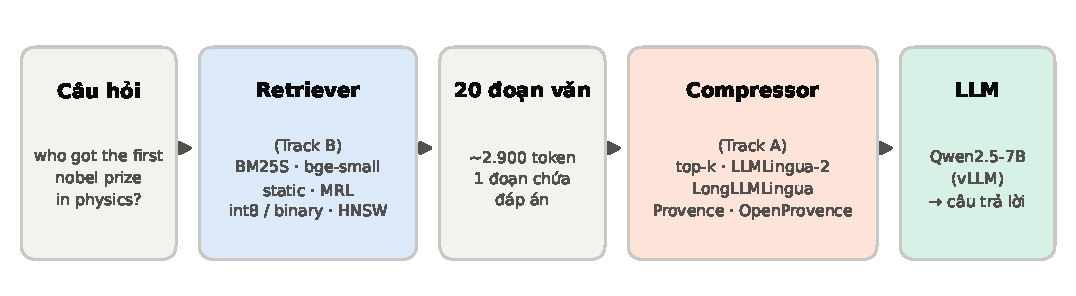
\includegraphics[width=\linewidth]{pipeline.pdf}}{\fbox{pipeline}}
\caption{Pipeline Efficient RAG: truy hồi $\rightarrow$ nén ngữ cảnh $\rightarrow$ sinh câu trả lời.
Track A đánh giá khối nén (với 20 đoạn cho sẵn), Track B đánh giá khối truy hồi.}
\label{fig:pipeline}
\end{figure}

\subsection{Các phương pháp nén ngữ cảnh}
\label{sec:compressors}

Chúng tôi chia các bộ nén thành bốn nhóm theo đơn vị bị loại bỏ (Bảng~\ref{tab:compressors}).

\paragraph{Tham chiếu.} \emph{Closed-book} (không ngữ cảnh) là cận dưới; \emph{Oracle} (chỉ đoạn vàng)
là cận trên thực tế; \emph{Full} (giữ nguyên 20 đoạn) là baseline cần vượt qua.

\paragraph{Mức prompt -- Truncate.} Giữ $B$ token đầu tiên của ngữ cảnh đầy đủ. Đây là cách ``ngây thơ''
nhất để đạt một ngân sách token; nó loại bỏ hoàn toàn các đoạn ở cuối.

\paragraph{Mức tài liệu -- Top-$k$ selection.} Chấm điểm từng đoạn theo câu hỏi rồi giữ $k$ đoạn có
điểm cao nhất, \emph{giữ nguyên thứ tự ban đầu}. Ba bộ chấm điểm: BM25 (thưa, từ vựng), bi-encoder
\texttt{bge-small-en-v1.5}~\cite{xiao2024cpack} (cosine), và cross-encoder \texttt{ms-marco-MiniLM-L6-v2}
(reranker). Với 20 đoạn trung bình $\sim$2.900 token, $k=10$ và $k=5$ tương ứng nén khoảng 2$\times$ và
4$\times$, khớp với hai mức ngân sách trong bảng của LongLLMLingua.

\paragraph{Mức token.} \textbf{LLMLingua-2}~\cite{pan2024llmlingua2}: bộ phân loại token
XLM-RoBERTa-large dự đoán xác suất giữ $p(\text{keep}\mid x_i)$; giữ các token có xác suất cao nhất
sao cho đạt tỉ lệ $r$ (ngưỡng toàn cục trên cả 20 đoạn). \textbf{LongLLMLingua}~\cite{jiang2024longllmlingua}:
tính perplexity có điều kiện câu hỏi bằng LM nhân quả nhỏ (Qwen2.5-0.5B-Instruct thay cho Llama-2-7B
trong bài gốc) để xếp hạng đoạn và nén token với ngân sách $B$ token. Ngoài ra, chúng tôi ghép
\textbf{reranker top-10 $\rightarrow$ LLMLingua-2 ($r=0{,}5$)} để mô phỏng chiến lược coarse-to-fine.

\paragraph{Mức câu -- Context pruning.} \textbf{Provence}~\cite{chirkova2025provence} là một cross-encoder
DeBERTa-v3-large với hai đầu ra: điểm liên quan của cả đoạn (reranking) và xác suất giữ của từng token,
được gộp thành quyết định giữ/bỏ từng \emph{câu} theo ngưỡng $\tau$. Ngưỡng nhỏ giữ nhiều câu hơn.
Đoạn không còn câu nào bị loại hẳn. \textbf{OpenProvence}~\cite{openprovence} dùng cùng ý tưởng với
backbone ModernBERT-base (150M tham số, nhỏ hơn 3 lần). Chúng tôi quét $\tau\in\{0{,}01; 0{,}1; 0{,}5\}$
cho Provence và $\tau\in\{0{,}1; 0{,}5\}$ cho OpenProvence.

\begin{table}[t]
\centering
\caption{Các bộ nén được đánh giá. ``Hỏi'' = có dùng câu hỏi khi nén.}
\label{tab:compressors}
\small
\begin{tabular}{l l l c r}
\toprule
Nhóm & Phương pháp & Mô hình & Hỏi & Tham số \\
\midrule
Tham chiếu & Closed-book / Oracle / Full & -- & -- & -- \\
Prompt & Truncate & -- & -- & 0 \\
Tài liệu & BM25 top-$k$ & BM25S & \checkmark & 0 \\
 & Dense top-$k$ & bge-small-en-v1.5 & \checkmark & 33M \\
 & Rerank top-$k$ & ms-marco-MiniLM-L6-v2 & \checkmark & 23M \\
Token & LLMLingua-2 & xlm-roberta-large & -- & 559M \\
 & LongLLMLingua & Qwen2.5-0.5B-Instruct & \checkmark & 494M \\
 & Rerank $\rightarrow$ LLMLingua-2 & MiniLM + XLM-R & \checkmark & 582M \\
Câu & Provence & deberta-v3-large & \checkmark & 435M \\
 & OpenProvence & gte-modernbert-base & \checkmark & 150M \\
\bottomrule
\end{tabular}
\end{table}

\paragraph{Tính bất biến theo thứ tự.} Các bộ nén mức tài liệu, mức câu và LLMLingua-2 xử lý từng đoạn
độc lập với vị trí của nó. Chúng tôi tận dụng tính chất này: kết quả nén của một tập đoạn được ghi nhớ
và tái sử dụng cho năm vị trí đoạn vàng (chỉ thứ tự thay đổi), giảm 5 lần thời gian nén; độ trễ báo cáo
là độ trễ đo ở lần tính đầu tiên. Sau khi nén, các đoạn còn lại \emph{giữ nguyên thứ tự} và được đánh
số lại, nhờ đó biến ``vị trí đoạn vàng'' vẫn có ý nghĩa, giống thiết lập của các bảng đã công bố.

\subsection{Các phương pháp truy hồi hiệu quả}

Trên kho gộp $\sim$50,7 nghìn đoạn, chúng tôi so sánh:
\begin{itemize}
  \item \textbf{BM25S}~\cite{lu2024bm25s} với stemming và loại stopword.
  \item \textbf{Static embedding} \texttt{static-retrieval-mrl-en-v1}~\cite{hfstatic2025} (không có
  Transformer, 1024 chiều, hỗ trợ Matryoshka).
  \item \textbf{bge-small-en-v1.5} (33M, 384 chiều) với chỉ mục chính xác (flat), xấp xỉ (HNSW, $M=32$),
  lượng tử int8 và nhị phân.
  \item \textbf{Qwen3-Embedding-0.6B}~\cite{zhang2025qwen3emb} (1024 chiều) với cắt Matryoshka
  1024/256/64 chiều và lượng tử int8/nhị phân.
\end{itemize}
Lượng tử int8 ánh xạ tuyến tính mỗi chiều về 256 mức (theo min/max trên kho). Lượng tử nhị phân giữ
dấu của từng chiều (1 bit), tìm kiếm bằng khoảng cách Hamming trên $4k$ ứng viên, sau đó \emph{rescore}
bằng tích vô hướng giữa vector truy vấn float và vector tài liệu $\{-1,+1\}$~\cite{hfquant2024} -- không
cần lưu vector float của kho.

\subsection{Giao thức đánh giá}
\label{sec:protocol}

\paragraph{Dữ liệu.} 500 câu hỏi lấy ngẫu nhiên (seed 42) từ 2.655 câu của NQ-Open 20 tài liệu; cùng
500 câu cho cả năm vị trí đoạn vàng (1, 5, 10, 15, 20), tổng 2.500 prompt cho mỗi cấu hình.

\paragraph{Prompt.} Dùng nguyên mẫu prompt của \citet{liu2024lost}:
\begin{lstlisting}
Write a high-quality answer for the given question using only the provided search
results (some of which might be irrelevant).

Document [1](Title: ...) ...
...
Question: {question}
Answer:
\end{lstlisting}

\paragraph{Chỉ số.}
\begin{itemize}
  \item \textbf{Accuracy}: câu trả lời đúng nếu một trong các đáp án chuẩn (sau chuẩn hoá chữ thường,
  bỏ dấu câu và mạo từ) xuất hiện trong output -- định nghĩa của \citet{liu2024lost}, cũng được dùng
  bởi LongLLMLingua và LLMLingua-2.
  \item \textbf{Context recall}: đáp án còn xuất hiện trong ngữ cảnh sau nén hay không -- đo khả năng
  ``giữ bằng chứng'' độc lập với LLM.
  \item \textbf{Token và tỉ lệ nén}: đếm bằng một bộ tách từ chung (tiktoken \texttt{o200k\_base}) cho
  mọi phương pháp; tỉ lệ nén $=$ token gốc / token sau nén.
  \item \textbf{Độ trễ}: thời gian nén mỗi câu hỏi và thời gian gọi LLM.
  \item Truy hồi: \textbf{answer-hit@$k$} (top-$k$ chứa đáp án, như DPR~\cite{karpukhin2020dpr}),
  \textbf{MRR@10} của đoạn vàng, kích thước chỉ mục, thời gian truy vấn.
\end{itemize}

\section{Cài đặt hệ thống}
\label{sec:impl}

\subsection{Tổ chức mã nguồn}

Toàn bộ mã nguồn được công khai tại \url{https://github.com/hotamago/nlp-efficient-rag}, viết bằng
Python 3.11 và quản lý môi trường bằng \texttt{uv} (khoá phiên bản trong \texttt{uv.lock}). Gói
\texttt{effrag} gồm các mô-đun:

\begin{itemize}
  \item \texttt{data.py}: đọc bộ NQ-Open 20 tài liệu, lấy mẫu cố định theo seed, gộp kho truy hồi.
  \item \nolinkurl{compression/}: lớp trừu tượng \texttt{Compressor} và \texttt{DocwiseCompressor}
  (ghi nhớ kết quả theo tập tài liệu), các bộ nén ở Bảng~\ref{tab:compressors} và bộ ghép
  \texttt{Chain} (nén nhiều tầng).
  \item \texttt{retrieval.py}: \texttt{BM25Retriever} và \texttt{DenseRetriever} (cắt Matryoshka,
  lượng tử int8/nhị phân, chỉ mục flat/HNSW).
  \item \texttt{generation.py}: client tương thích OpenAI, có cache theo hash của prompt và thử lại
  khi lỗi; cùng một mã chạy được với API thương mại, vLLM hoặc Ollama.
  \item \texttt{metrics.py}, \texttt{tokens.py}, \texttt{results.py}: chỉ số, bộ đếm token chung và
  lược đồ kết quả (CSV/JSONL) dùng chung cho cả nhóm.
  \item \nolinkurl{scripts/}: chạy thí nghiệm (\texttt{run\_compression.py}, \texttt{run\_retrieval.py},
  \nolinkurl{run_all_compression.sh}), vẽ hình (\texttt{make\_figures.py}); \nolinkurl{app/demo.py}: demo Gradio.
\end{itemize}

Thêm một bộ nén mới chỉ cần kế thừa \texttt{Compressor} và cài đặt một hàm:
\begin{lstlisting}[language=Python]
class MyPruner(DocwiseCompressor):
    name = "my_pruner"
    def _compress_docs(self, question, docs):   # -> one string per document ("" = drop)
        return [prune(question, d) for d in docs]
\end{lstlisting}

\subsection{Thư viện, mô hình và dữ liệu sử dụng}

\begin{table}[h]
\centering
\caption{Thành phần có sẵn được sử dụng.}
\label{tab:libs}
\small
\begin{tabularx}{\linewidth}{l X}
\toprule
Thành phần & Phiên bản / nguồn \\
\midrule
Dữ liệu & NQ-Open multi-document QA, 20 tài liệu~\cite{liu2024lost} (\nolinkurl{nelson-liu/lost-in-the-middle}) \\
LLM sinh câu trả lời & \nolinkurl{Qwen/Qwen2.5-7B-Instruct-AWQ}~\cite{qwen2025qwen25,lin2024awq}, phục vụ bằng vLLM 0.31~\cite{kwon2023vllm} \\
Nén token & \texttt{llmlingua} 0.2.2; \nolinkurl{microsoft/llmlingua-2-xlm-roberta-large-meetingbank}; \nolinkurl{Qwen/Qwen2.5-0.5B-Instruct} \\
Nén câu & \nolinkurl{naver/provence-reranker-debertav3-v1}; \nolinkurl{hotchpotch/open-provence-reranker-v1-gte-modernbert-base} \\
Truy hồi & \texttt{bm25s} 0.3, \texttt{faiss-cpu} 1.15, \texttt{sentence-transformers} 5.7; \nolinkurl{BAAI/bge-small-en-v1.5}, \nolinkurl{static-retrieval-mrl-en-v1}, \nolinkurl{cross-encoder/ms-marco-MiniLM-L6-v2} \\
Nền tảng & PyTorch 2.14, Transformers 4.57, tiktoken 0.14, Gradio 6 \\
\bottomrule
\end{tabularx}
\end{table}

\subsection{Thông số thực nghiệm}

\begin{itemize}
  \item \textbf{Phần cứng}: 1 GPU NVIDIA RTX 4070 SUPER 12GB, CPU 20 luồng (mặc định 4 luồng cho mỗi
  tiến trình, 8 luồng khi đo độ trễ CPU), 24GB RAM, WSL2.
  \item \textbf{Sinh câu trả lời}: Qwen2.5-7B-Instruct (lượng tử AWQ 4-bit), \texttt{temperature}=0,
  tối đa 100 token sinh (như \citet{liu2024lost}), độ dài ngữ cảnh tối đa 4.096 token.
  \item \textbf{Lấy mẫu}: 500 câu hỏi, seed 42, 3 vị trí đoạn vàng $\{1,10,20\}$.
  \item \textbf{Ngân sách nén}: tương ứng 2$\times$ ($\approx$1.450 token) và 4$\times$ ($\approx$730 token)
  so với $\approx$2.900 token của ngữ cảnh đầy đủ -- cùng hai mức của bảng kết quả LongLLMLingua.
  \item \textbf{LongLLMLingua}: \nolinkurl{condition_compare=True}, \nolinkurl{condition_in_question="after"},
  \nolinkurl{rank_method="longllmlingua"}, \nolinkurl{dynamic_context_compression_ratio=0.4},
  \nolinkurl{context_budget="+100"}, \nolinkurl{reorder_context="original"}.
  \item \textbf{LLMLingua-2}: \texttt{rate}$\in\{0{,}5; 0{,}25\}$, giữ bắt buộc ký tự xuống dòng, ``?'' và ``.''.
\end{itemize}

\paragraph{Điều chỉnh tương thích.} \texttt{llmlingua} 0.2.2 thao tác KV-cache dạng tuple cũ; chúng
tôi bọc hàm \texttt{forward} của LM để chuyển đổi qua lại với \texttt{DynamicCache} của Transformers
mới. Các mô hình Provence dùng mã tuỳ biến (\texttt{trust\_remote\_code}); với OpenProvence, mỗi cặp
(câu hỏi, đoạn) được đưa vào như một phần tử độc lập của batch.

\subsection{Demo}
\label{sec:demo}

\nolinkurl{app/demo.py} là ứng dụng Gradio chỉ gọi API của gói \texttt{effrag} (không sao chép logic),
gồm hai tab:
\begin{itemize}
  \item \textbf{So sánh bộ nén}: chọn một câu hỏi trong 200 câu đầu, vị trí đoạn vàng và các bộ nén;
  ứng dụng hiển thị số token trước/sau nén, thời gian nén, đáp án còn trong ngữ cảnh hay không và
  câu trả lời của LLM (Hình~\ref{fig:demo}). Với bộ nén theo đoạn, từng câu được giữ được tô xanh,
  câu bị loại bị gạch, đoạn vàng được đánh dấu (Hình~\ref{fig:demo-context}).
  \item \textbf{RAG end-to-end}: câu hỏi tự do $\to$ BM25S hoặc bge-small trên kho 50,7k đoạn
  $\to$ bộ nén $\to$ LLM.
\end{itemize}
Khi không có máy chủ LLM, demo vẫn chạy phần truy hồi và nén; mọi mô hình nén chạy được trên CPU
(\texttt{EFFRAG\_DEVICE=cpu}). Ảnh chụp dưới đây được lấy khi chạy toàn bộ bộ nén trên CPU (4 luồng, máy đang chạy job khác), LLM
qua vLLM.

\begin{figure}[t]
\centering
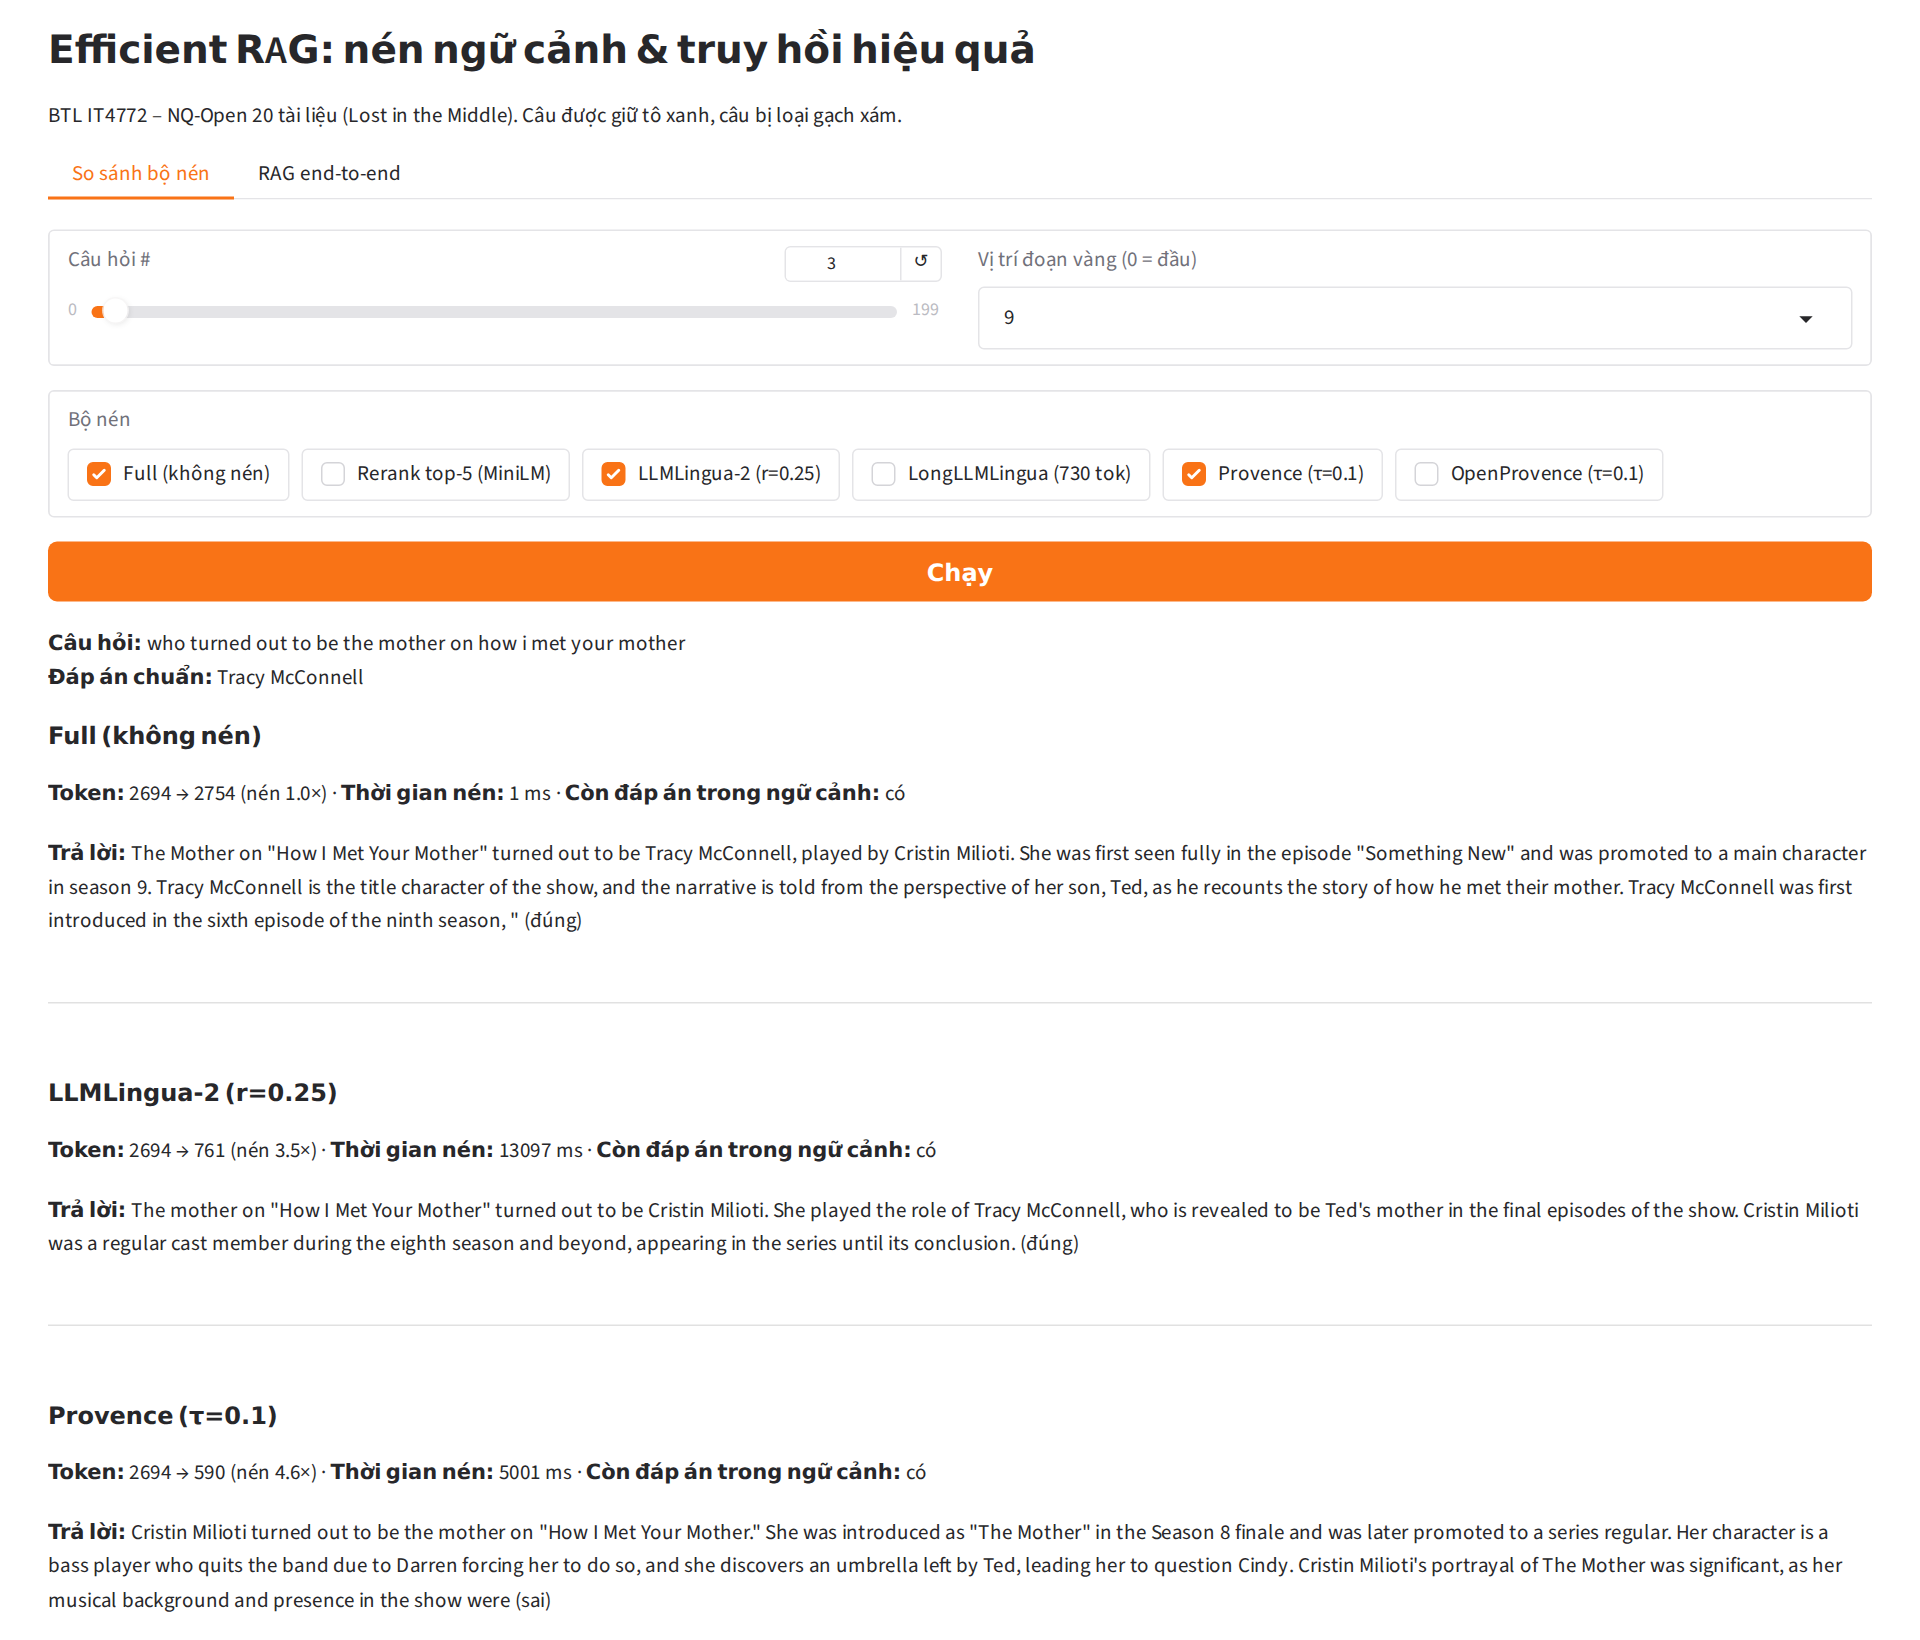
\includegraphics[width=\linewidth]{demo.png}
\caption{Tab ``So sánh bộ nén'' của demo (câu hỏi \#3, đoạn vàng ở vị trí 10, chạy trên CPU).
LLMLingua-2 và Provence đều giữ được đáp án; với Provence, reader 7B trả lời bằng tên diễn viên
(Cristin Milioti) thay vì tên nhân vật -- một kiểu lỗi được phân tích ở Mục~\ref{sec:res-errors}.}
\label{fig:demo}
\end{figure}

\begin{figure}[t]
\centering
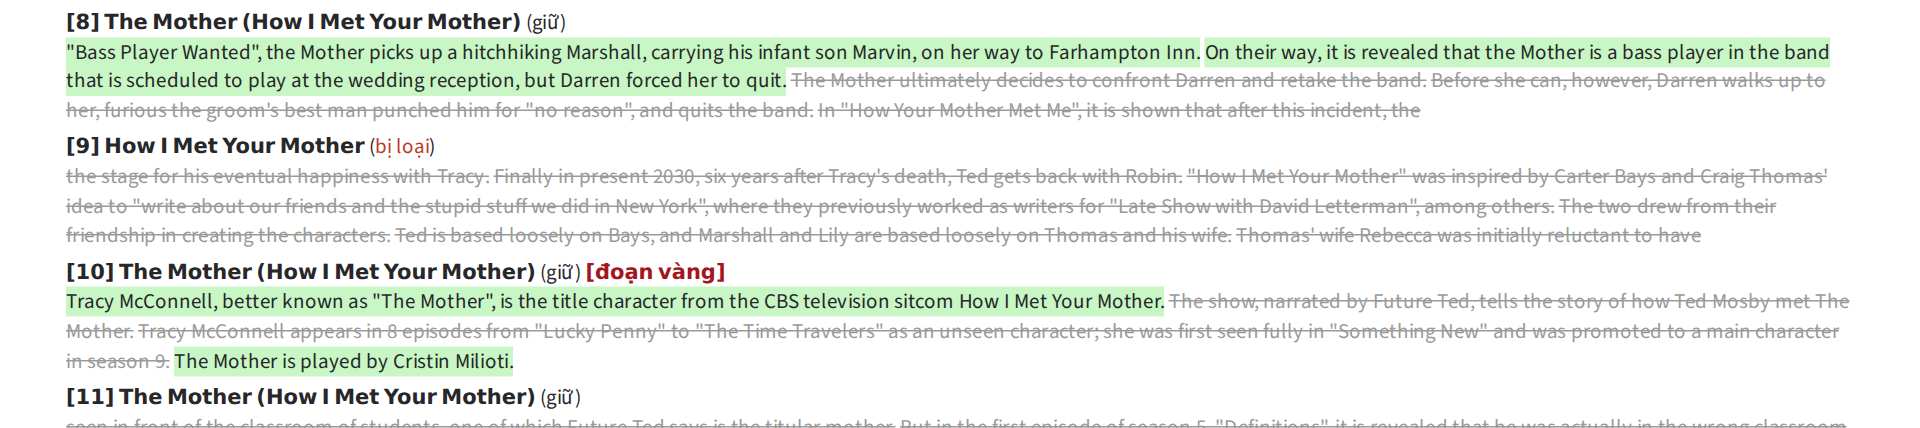
\includegraphics[width=\linewidth]{demo_context.png}
\caption{Ngữ cảnh sau nén của Provence trong demo: câu được giữ (nền xanh), câu bị loại (gạch ngang),
đoạn bị loại hoàn toàn và đoạn vàng.}
\label{fig:demo-context}
\end{figure}

\section{Kết quả và thảo luận}
\label{sec:results}

Mọi số liệu trong mục này được sinh tự động từ \texttt{results/} bằng
\texttt{scripts/make\_figures.py}; mỗi câu hỏi có một dòng trong các tệp \texttt{.jsonl} đã commit.
Trừ khi ghi chú khác, $n=500$ câu hỏi, các vị trí đoạn vàng 1/10/20, reader Qwen2.5-7B-Instruct-AWQ.

%------------------------------------------------------------------------------
\subsection{Bộ nén giữ được bao nhiêu bằng chứng?}
\label{sec:res-recall}

Bảng~\ref{tab:recall} đo \emph{context recall} -- tỉ lệ câu hỏi mà đáp án còn nằm trong ngữ cảnh sau
nén -- cho mọi bộ nén mà không cần gọi LLM. Đây là trần trên của độ chính xác sau nén: nếu đáp án đã bị
xoá thì reader chỉ còn trả lời được bằng tri thức tham số (closed-book).

\begin{table}[t]
\centering
\caption{Context recall (\%) theo vị trí đoạn vàng, số token sau nén, tỉ lệ nén và độ trễ nén trung
bình mỗi câu hỏi (GPU). Bộ nén mức tài liệu/token/câu xử lý từng đoạn độc lập nên recall không phụ
thuộc vị trí. LongLLMLingua: $n=200$, chỉ vị trí 10.}
\label{tab:recall}
\small
\begin{tabular}{l r r r r r r}
\toprule
Bộ nén & Token & Nén & R@1 & R@10 & R@20 & ms/câu \\
\midrule
\inputtable{tables/recall.tex}
\bottomrule
\end{tabular}
\end{table}

\paragraph{Nhận xét.}
\begin{itemize}
  \item \textbf{Ở cùng mức nén $\approx$4$\times$, nén mức câu giữ bằng chứng tốt nhất}: Provence
  ($\tau=0{,}1$) giữ 91,6\% đáp án với 621 token (4,6$\times$), hơn Rerank top-5 (79,4\%) 12,2 điểm,
  hơn LongLLMLingua (77,5\%) và LLMLingua-2 $r=0{,}25$ (68,0\%) lần lượt 14 và 24 điểm. Cắt tỉa theo
  \emph{câu}, có điều kiện câu hỏi, giữ nguyên các câu chứa đáp án; còn bỏ token rời rạc (LLMLingua-2
  không nhìn câu hỏi) có thể làm mất chính thực thể cần trả lời.
  \item \textbf{Ở $\approx$2$\times$}, OpenProvence (96,4\%, 2,6$\times$) và Provence $\tau=0{,}01$
  (95,8\%, 2,5$\times$) gần như không mất bằng chứng; Rerank top-10 (89,8\%) và LLMLingua-2 $r=0{,}5$
  (88,2\%) mất khoảng 10\%.
  \item \textbf{BM25 kém trong bối cảnh này} (53,2\% ở top-5): 19 đoạn nhiễu của bộ dữ liệu vốn được
  Contriever truy hồi là ``hard negative'' có độ trùng từ vựng cao với câu hỏi. Cross-encoder MiniLM
  (22M tham số), đọc câu hỏi và đoạn cùng lúc, cho recall cao hơn bi-encoder bge-small 10,4 điểm mà
  vẫn nhanh hơn (14 so với 121 ms mỗi câu trong cài đặt của chúng tôi).
  \item \textbf{Truncate} đúng như kỳ vọng: giữ trọn đáp án khi đoạn vàng ở đầu và mất gần hết khi đoạn
  vàng ở giữa/cuối -- một baseline cho thấy vì sao cần nén \emph{có điều kiện câu hỏi}.
\end{itemize}

%------------------------------------------------------------------------------
\subsection{Độ chính xác của RAG sau nén}
\label{sec:res-main}

\begin{table}[t]
\centering
\caption{Kết quả chính (Qwen2.5-7B-Instruct-AWQ, $n=500$): accuracy (\%) theo vị trí đoạn vàng và
trung bình (TB), số token ngữ cảnh, tỉ lệ nén, context recall (\%) và độ trễ nén (ms/câu, GPU). BM25 và
Dense top-5 chỉ chạy ở vị trí 10 (đã có số công bố, Mục~\ref{sec:res-published}); LongLLMLingua
($n=200$) ở Bảng~\ref{tab:published}. In đậm: TB cao nhất trong các bộ nén.}
\label{tab:main}
\small
\setlength{\tabcolsep}{4pt}
\begin{tabular}{l r r r r r r r r}
\toprule
Cấu hình & @1 & @10 & @20 & TB & Token & Nén & Recall & ms \\
\midrule
\inputtable{tables/main_results.tex}
\end{tabular}
\end{table}

\begin{figure}[t]
\centering
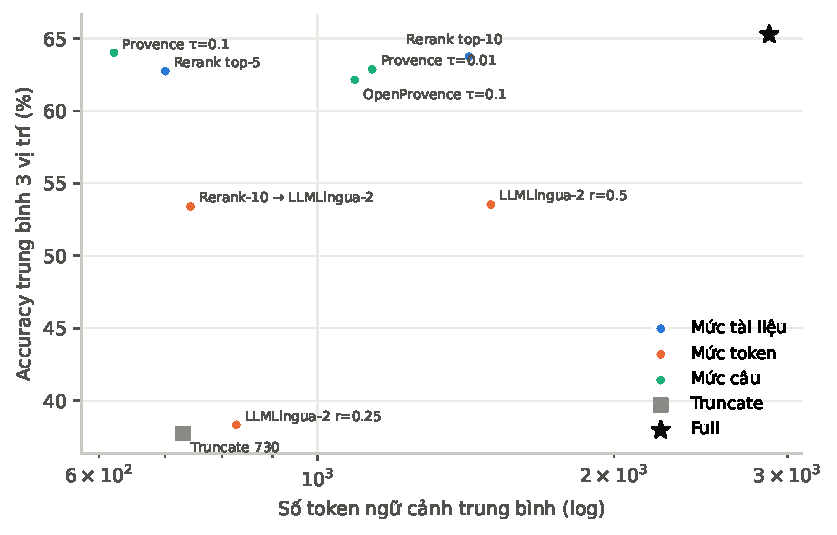
\includegraphics[width=0.8\linewidth]{tradeoff.pdf}
\caption{Accuracy trung bình 3 vị trí theo số token ngữ cảnh (thang log). Góc trên bên trái là tốt
nhất: ít token, độ chính xác cao.}
\label{fig:tradeoff}
\end{figure}

Bảng~\ref{tab:main} và Hình~\ref{fig:tradeoff} cho thấy khoảng cách giữa closed-book (38,8\%) và
oracle (92,6\%) là 53,8 điểm: ngữ cảnh rất quan trọng, nhưng 20 đoạn đầy đủ (65,3\%) chỉ khai thác được
một nửa khoảng cách đó vì nhiễu. Kiểm định bootstrap ghép cặp (10.000 lần lấy mẫu, khoảng tin cậy 95\%,
\texttt{results/compression/significance.csv}) so với ngữ cảnh đầy đủ cho các kết luận sau.

\begin{itemize}
  \item \textbf{Ở 4$\times$, nén mức câu gần như không mất độ chính xác.} Provence $\tau=0{,}1$ dùng
  621 token (4,6$\times$) và đạt 64,0\% so với 65,3\%; chênh lệch ở cả ba vị trí đều không có ý nghĩa
  thống kê ($-1{,}8$ [$-5{,}6$; $2{,}0$], $+0{,}4$ [$-3{,}4$; $4{,}2$], $-2{,}4$ [$-6{,}2$; $1{,}4$]
  điểm ở vị trí 1/10/20). Đây là cấu hình tốt nhất trên toàn bộ đường Pareto.
  \item \textbf{Chọn tài liệu bằng cross-encoder đứng thứ hai.} Rerank top-5 (4,1$\times$) đạt 62,7\%,
  nhưng giảm có ý nghĩa ở vị trí 20 ($-6{,}0$ [$-10{,}0$; $-2{,}2$]) vì 20,6\% câu mất đoạn chứa đáp án.
  Rerank top-10 (2$\times$) đạt 63,7\%. Bộ chọn rẻ hơn kém xa: Dense top-5 56,0\%, BM25 top-5 45,4\%
  (vị trí 10).
  \item \textbf{Nén mức token thất bại với reader 7B.} LLMLingua-2 $r=0{,}25$ (3,5$\times$) chỉ đạt
  38,3\% -- ngang closed-book -- dù context recall vẫn còn 68\%; ở $r=0{,}5$ (1,9$\times$) cũng chỉ
  53,5\%. Ghép rerank-10 trước LLMLingua-2 (cấu hình tốt nhất của LLMLingua-2 trên GPT-3.5) đạt 53,4\%,
  giảm có ý nghĩa ở mọi vị trí. Mục~\ref{sec:res-errors} cho thấy phần lớn thiệt hại không đến từ việc
  xoá đáp án mà từ việc văn bản bị xé vụn khiến reader đọc sai.
  \item \textbf{OpenProvence} (2,6$\times$) giữ bằng chứng tốt nhất (recall 96,4\%) nhưng accuracy
  62,1\%, thấp hơn Provence $\tau=0{,}1$ dù giữ nhiều token hơn: giữ thêm câu nhiễu không giúp reader.
  \item \textbf{Truncate} là trường hợp đặc biệt: khi đoạn vàng ở đầu, cắt còn 730 token lại
  \emph{tăng} accuracy lên 74,0\% ($+8{,}4$ [$5{,}0$; $12{,}0$]) vì loại bỏ 15 đoạn nhiễu; nhưng ở vị trí
  10/20 chỉ còn 19,6\%. Điều này xác nhận rằng ngữ cảnh ngắn và đúng tốt hơn ngữ cảnh dài -- vấn đề là
  chọn \emph{đúng} phần nào.
\end{itemize}

\paragraph{Chi phí.} Với vLLM, thời gian prefill tỉ lệ với số token: Provence giảm 2.875 $\to$ 621 token
mỗi câu, đổi lại khoảng 200 ms nén trên GPU (4,9 s trên CPU, Bảng~\ref{tab:latency}). Rerank top-5
rẻ hơn hẳn (16 ms GPU, 196 ms CPU) với độ chính xác thấp hơn 1,3 điểm -- là lựa chọn hợp lý khi không có
GPU.

%------------------------------------------------------------------------------
\subsection{Nén và hiện tượng \emph{lost in the middle}}
\label{sec:res-position}

\begin{figure}[t]
\centering
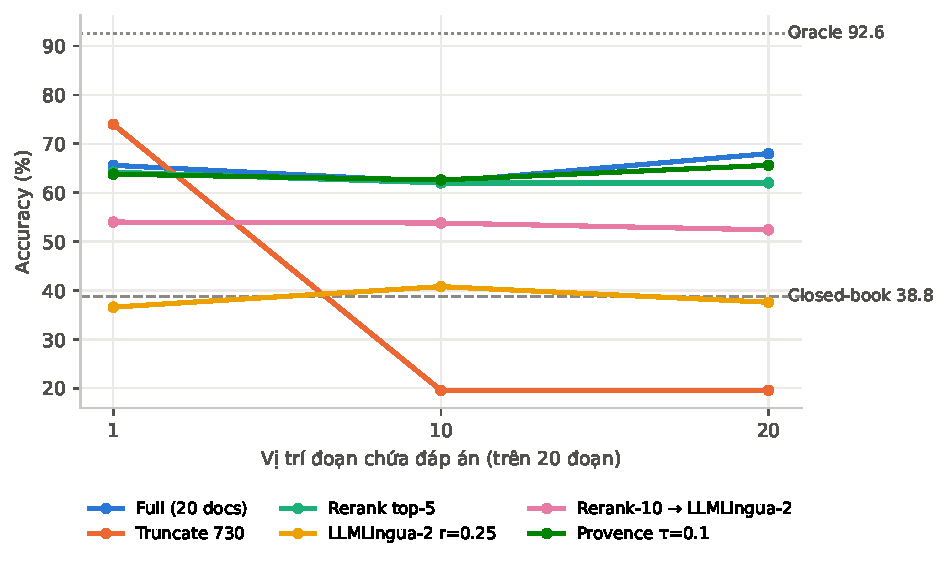
\includegraphics[width=0.8\linewidth]{position_curve.pdf}
\caption{Accuracy theo vị trí đoạn chứa đáp án. Đường ngang: closed-book và oracle.}
\label{fig:position}
\end{figure}

Với GPT-3.5-Turbo, \citet{liu2024lost} và LongLLMLingua báo cáo đường cong chữ U sâu: 75,7 / 54,1 /
63,1\% ở vị trí 1/10/20, chênh 21,6 điểm giữa đầu và giữa. Với Qwen2.5-7B-Instruct, đường cong của ngữ
cảnh đầy đủ gần như phẳng (65,6 / 62,2 / 68,0\%): chênh lệch lớn nhất chỉ 5,8 điểm, và vị trí cuối còn
tốt hơn vị trí đầu (Hình~\ref{fig:position}). Các mô hình mới được huấn luyện với ngữ cảnh dài hơn
nhiều (Qwen2.5: 32K--128K token) nên 2.900 token không còn là ngữ cảnh ``dài''.

Hệ quả là nén \emph{không có nhiều chỗ để làm phẳng} đường cong: Provence $\tau=0{,}1$ cho 63,8 / 62,6 /
65,6\%, gần như song song với ngữ cảnh đầy đủ. Các bộ nén không phụ thuộc vị trí (mức tài liệu, câu,
token) giữ nguyên hình dạng đường cong của reader; chỉ truncate -- vốn phụ thuộc vị trí -- tạo ra độ
dốc lớn.

%------------------------------------------------------------------------------
\subsection{Đối chiếu với số liệu đã công bố}
\label{sec:res-published}

\begin{table}[t]
\centering
\caption{So sánh với số liệu đã công bố trên cùng benchmark (GPT-3.5-Turbo-0613; LongLLMLingua
\citep{jiang2024longllmlingua} Bảng 1 và LLMLingua-2 \citep{pan2024llmlingua2} Bảng 4). Hàng đầu:
accuracy tuyệt đối (\%) của ngữ cảnh đầy đủ; các hàng sau: \emph{chênh lệch} (điểm) so với ngữ cảnh
đầy đủ của chính hệ đó. LongLLMLingua của chúng tôi: so cặp trên 193 câu chung với lần chạy đầy đủ.}
\label{tab:published}
\small
\setlength{\tabcolsep}{3.5pt}
\begin{tabular}{l r r r l r r r}
\toprule
\multicolumn{4}{c}{GPT-3.5-Turbo (đã công bố)} & \multicolumn{4}{c}{Qwen2.5-7B-AWQ (của chúng tôi)} \\
\cmidrule(lr){1-4}\cmidrule(lr){5-8}
Phương pháp & @1 & @10 & @20 & Cấu hình tương ứng & @1 & @10 & @20 \\
\midrule
\inputtable{tables/published.tex}
\bottomrule
\end{tabular}
\end{table}

Vì GPT-3.5-Turbo-0613 đã ngừng hoạt động, chúng tôi so sánh \emph{độ chênh so với baseline của chính
mỗi hệ} (Bảng~\ref{tab:published}) thay vì số tuyệt đối.
\begin{itemize}
  \item \textbf{Tái lập được}: thứ hạng giữa các bộ chọn tài liệu (SBERT/Dense tốt hơn BM25 rõ rệt) và
  mức sụt nặng của LLMLingua-2 đơn lẻ ở 4$\times$ ($-29{,}0$ / $-21{,}4$ / $-30{,}4$ điểm so với
  $-27{,}1$ / $-10{,}5$ / $-23{,}2$ được công bố).
  \item \textbf{Không tái lập được}: kết luận ``nén làm \emph{tăng} độ chính xác ở giữa'' -- LongLLMLingua
  $+17{,}1$ và LLMLingua-2 + lọc tài liệu $+12{,}9$ điểm ở vị trí 10. Với reader của chúng tôi, mức thay
  đổi tương ứng là $+1{,}0$ (không có ý nghĩa thống kê, khoảng tin cậy [$-6{,}7$; $8{,}8$]) và $-8{,}4$.
  Lời giải thích hợp lý nhất là ở Mục~\ref{sec:res-position}: lợi ích chính của các phương pháp này trên
  GPT-3.5 là \emph{khắc phục lost in the middle}, mà reader hiện đại hầu như không còn mắc.
  \item Về vị trí đầu và cuối, cả hai hệ đều cho thấy nén 4$\times$ ở mức tốt nhất chỉ \emph{hoà}
  với ngữ cảnh đầy đủ (LongLLMLingua $-0{,}7$ trên GPT-3.5; Provence $-1{,}8$ / $-2{,}4$ của chúng tôi).
\end{itemize}

%------------------------------------------------------------------------------
\subsection{Nén mềm}
\label{sec:res-soft}

\begin{table}[t]
\centering
\caption{Nén mềm so với văn bản trên \emph{cùng} một reader (accuracy \%, 500 câu/vị trí; rerank: chỉ
vị trí 10). Token: số vector nhớ hoặc token văn bản đưa vào reader; Nén: so với 20 đoạn văn bản.}
\label{tab:soft}
\small
\begin{tabular}{l r r r r r r}
\toprule
Cấu hình & @1 & @10 & @20 & TB & Token & Nén \\
\midrule
\inputtable{tables/soft.tex}
\end{tabular}
\end{table}

% TODO(T09): text for PISCO (T12) + own encode-once model (T16-T18)

%------------------------------------------------------------------------------
\subsection{Truy hồi hiệu quả}
\label{sec:res-retrieval}

Bảng~\ref{tab:retrieval} so sánh các retriever trên kho gộp 50,7k đoạn (mọi đoạn của 2.655 câu hỏi),
với 500 câu hỏi của tập đánh giá.

\begin{table}[t]
\centering
\caption{Truy hồi trên kho 50,7k đoạn ($n=500$). Hit@$k$: top-$k$ chứa đoạn có đáp án (\%); MRR@10
của đoạn vàng (\%); kích thước chỉ mục (MB); thời gian truy vấn mỗi câu khi chạy theo batch và khi
chạy từng câu (ms, GPU cho mô hình nhúng).}
\label{tab:retrieval}
\small
\begin{tabular}{l r r r r r r r}
\toprule
Hệ thống & Hit@1 & Hit@5 & Hit@20 & MRR@10 & MB & ms (batch) & ms (1 câu) \\
\midrule
\inputtable{tables/retrieval.tex}
\bottomrule
\end{tabular}
\end{table}

\begin{figure}[t]
\centering
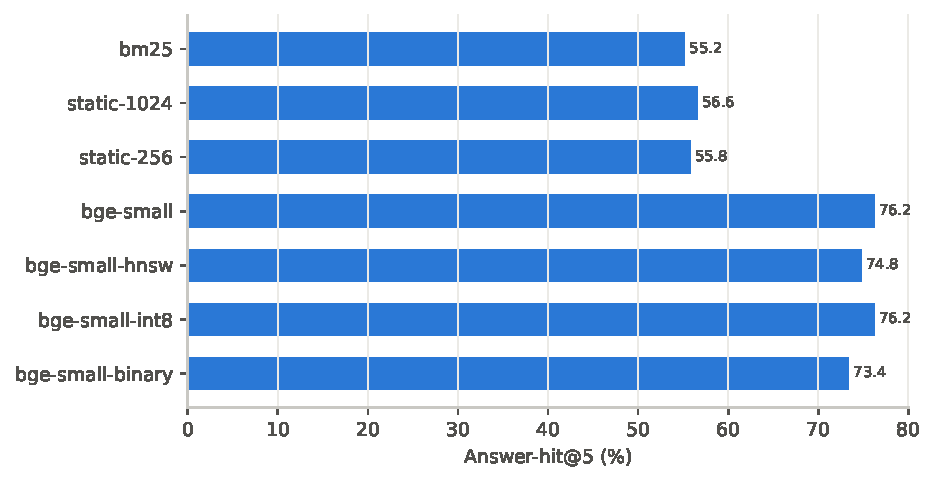
\includegraphics[width=0.75\linewidth]{retrieval_hit5.pdf}
\caption{Answer-hit@5 của các retriever trên kho 50,7k đoạn.}
\label{fig:retrieval}
\end{figure}

\paragraph{Nhận xét.}
\begin{itemize}
  \item \textbf{Retriever dày đặc nhỏ vượt xa BM25}: bge-small (33M) đạt hit@5 76,2\% so với 55,2\%
  của BM25S, MRR@10 53,8 so với 31,6.
  \item \textbf{Lượng tử int8 miễn phí}: chỉ mục giảm 4$\times$ (74,3 $\to$ 18,6 MB) mà hit@5 giữ
  nguyên 76,2\%; MRR@10 chỉ giảm 0,1 điểm.
  \item \textbf{Nhị phân + rescore}: chỉ mục 2,3 MB (32$\times$ nhỏ hơn) vẫn đạt 73,4\% hit@5 (mất 2,8
  điểm), hit@20 gần như không đổi (94,4 so với 95,4) -- phù hợp làm tầng truy hồi đầu, sau đó rerank.
  \item \textbf{Static embedding} (không có Transformer) ngang BM25 về chất lượng (55,8--56,6\%) và
  không cần GPU; cắt Matryoshka 1024 $\to$ 256 chiều giảm chỉ mục 4$\times$ chỉ mất 0,8 điểm hit@5.
  \item HNSW giảm độ trễ truy vấn đơn (12,6 $\to$ 5,5 ms) đổi lấy 1,4 điểm hit@5; ở quy mô 50k đoạn,
  tìm kiếm chính xác vẫn đủ nhanh.
\end{itemize}

%------------------------------------------------------------------------------
\subsection{Chạy không cần GPU}
\label{sec:res-cpu}

\begin{table}[t]
\centering
\caption{Độ trễ nén (trung vị ms/câu, 20 câu ở vị trí 10, gọi từng câu một sau 1 lần khởi động; không
tính LLM). GPU: RTX 4070 SUPER 12 GB; CPU: Core i5-14600K, 8 luồng.}
\label{tab:latency}
\small
\begin{tabular}{l r r r}
\toprule
Bộ nén & GPU (ms) & CPU (ms) & CPU/GPU \\
\midrule
\inputtable{tables/latency.tex}
\bottomrule
\end{tabular}
\end{table}

Câu hỏi thực tế của nhóm là: nếu không có GPU, phần nào của pipeline còn dùng được? Reader được gọi
qua API tương thích OpenAI (vLLM cục bộ hoặc dịch vụ trả phí), nên phần chạy cục bộ chỉ còn bộ nén.
Bảng~\ref{tab:latency} cho thấy ba nhóm rõ rệt:
\begin{itemize}
  \item \textbf{Mức tài liệu} (BM25, dense, rerank) chạy dưới 0,4 s/câu trên CPU -- đủ cho ứng dụng
  tương tác. Rerank top-5 (196 ms) giữ 62,7\% accuracy trung bình so với 65,3\% của ngữ cảnh đầy đủ ở
  4,1$\times$.
  \item \textbf{Mức câu} (OpenProvence, Provence) chậm 21--25$\times$ khi chuyển sang CPU: 1,6 s và 4,9
  s/câu. Provence là bộ nén tốt nhất về accuracy nhưng chỉ phù hợp xử lý theo lô hoặc khi độ trễ vài
  giây chấp nhận được; OpenProvence (ModernBERT-base, nhỏ hơn) nhanh gấp 3 lần trên CPU.
  \item \textbf{Mức token} (LLMLingua-2, LongLLMLingua) chậm nhất: 13--15 s/câu trên CPU, trong khi
  accuracy cũng kém hơn (Mục~\ref{sec:res-main}). Không có lý do dùng chúng khi không có GPU.
\end{itemize}

Khi reader là API tính phí theo token, nén 4,6$\times$ bằng Provence giảm 78\% token ngữ cảnh đầu
vào (2.875 $\to$ 621) với accuracy giảm 1,3 điểm (không có ý nghĩa thống kê). Như vậy toàn bộ hệ thống
-- bộ nén trên CPU, reader qua API -- chạy được không cần GPU; GPU chỉ rút ngắn độ trễ của các bộ nén dùng mô hình 12--29 lần.
Các bộ nén trong demo (Mục~\ref{sec:demo}) chạy trên CPU theo đúng cấu hình này.

%------------------------------------------------------------------------------
\subsection{Phân tích lỗi}
\label{sec:res-errors}

Với mỗi bộ nén và mỗi vị trí, chúng tôi ghép từng câu hỏi với kết quả của ngữ cảnh đầy đủ
(\texttt{scripts/error\_analysis.py}) và chia thành: \emph{hỏng do mất bằng chứng} (đầy đủ trả lời
đúng, sau nén sai và đáp án không còn trong ngữ cảnh), \emph{hỏng dù còn bằng chứng}, và \emph{được sửa}
(đầy đủ sai, sau nén đúng).

\begin{table}[t]
\centering
\caption{Phân loại thay đổi so với ngữ cảnh đầy đủ (\% số cặp câu hỏi--vị trí; 1.500 cặp, BM25/Dense
500 cặp). ``Sai, còn BC'': tỉ lệ câu sai sau nén dù đáp án vẫn còn trong ngữ cảnh.}
\label{tab:errors}
\small
\begin{tabular}{l r r r r r}
\toprule
Bộ nén & Hỏng, mất BC & Hỏng, còn BC & Được sửa & Ròng & Sai, còn BC \\
\midrule
\inputtable{tables/errors.tex}
\bottomrule
\end{tabular}
\end{table}

\begin{itemize}
  \item \textbf{Mọi bộ nén đều sửa được 5--9\% câu} mà ngữ cảnh đầy đủ trả lời sai: bớt nhiễu giúp reader
  tập trung. Với Provence $\tau=0{,}1$, số câu được sửa (8,8\%) gần bù hết số câu hỏng (10,1\%).
  \item \textbf{Nén mức câu gần như không xoá bằng chứng} (Provence 1,7\%, OpenProvence 0,3\%); phần
  hỏng chủ yếu là reader trả lời sai dù bằng chứng còn, thường vì câu bị cắt mất ngữ cảnh xung quanh.
  Ví dụ câu \emph{``who turned out to be the mother on how i met your mother''} (đáp án Tracy McConnell):
  sau nén, reader trả lời tên diễn viên (Cristin Milioti) thay vì tên nhân vật (Hình~\ref{fig:demo}).
  \item \textbf{LLMLingua-2 hỏng chủ yếu \emph{dù còn bằng chứng}}: ở $r=0{,}5$, 14,3\% so với 3,9\% do
  mất bằng chứng; ở $r=0{,}25$, 19,0\% so với 13,1\%. Văn bản bị bỏ token rời rạc (mất mạo từ, giới từ,
  dấu câu) vẫn chứa đáp án nhưng reader 7B không còn đọc đúng quan hệ giữa các thực thể.
  \item \textbf{Truncate và BM25 hỏng do mất bằng chứng} (27,7\% và 19,0\%).
  \item \textbf{Một phần lỗi do cách chấm}: reader 7B trả lời dài (tối đa 100 token) và đổi định dạng,
  ví dụ ``September 8, 2010'' bị chấm sai với đáp án ``8 September 2010''. Lỗi này ảnh hưởng như nhau
  đến mọi cấu hình nên không làm sai lệch so sánh, nhưng làm accuracy tuyệt đối thấp hơn thực tế.
\end{itemize}

\section{Kết luận}
\label{sec:conclusion}

\subsection{Trả lời câu hỏi nghiên cứu}

\begin{description}[leftmargin=2.6em,labelindent=0pt]
  \item[RQ1.] Ở mức nén $\approx$4$\times$, \textbf{chọn lọc theo câu} (Provence $\tau=0{,}1$, 4,6$\times$)
  là cách duy nhất không làm giảm accuracy có ý nghĩa thống kê ở cả ba vị trí (64,0\% so với 65,3\%
  của ngữ cảnh đầy đủ). Chọn lọc theo tài liệu (rerank top-5) rẻ hơn nhiều nhưng mất 2,6 điểm và giảm
  có ý nghĩa khi đoạn vàng ở cuối. Xoá theo token (LLMLingua-2 r=0,25) làm accuracy rơi về mức
  closed-book (38,3\% so với 38,8\%): phân tích lỗi cho thấy phần lớn thiệt hại đến từ văn bản bị xé
  vụn chứ không phải mất đáp án. Với reader hiện đại, đường cong vị trí vốn đã gần phẳng (chênh 5,8
  điểm) nên nén không còn tác dụng ``làm phẳng'' như báo cáo cho GPT-3.5.
  \item[RQ2.] Ở quy mô 50,7k đoạn, retriever dày đặc nhỏ (bge-small, 33M tham số) vượt BM25 21 điểm
  hit@5; lượng tử int8 giảm chỉ mục 4$\times$ không mất chất lượng, nhị phân + rescore giảm 32$\times$
  chỉ mất 2,8 điểm.
  \item[RQ3.] Tái lập được hai kết luận của các công bố: BM25 kém xa dense, và LLMLingua-2 dùng đơn lẻ
  ở 4$\times$ sụt mạnh ($-$21 đến $-$30 điểm so với $-$11 đến $-$27 được công bố). Không tái lập được
  kết luận ``nén làm tăng accuracy khi đoạn vàng ở giữa'' của LongLLMLingua ($+17{,}1$ điểm với GPT-3.5,
  $+1{,}0$ không có ý nghĩa với Qwen2.5-7B): hiệu ứng đó phụ thuộc vào reader bị \emph{lost in the
  middle}, điều không còn đúng với LLM mở thế hệ mới ở độ dài 3K token.
  \item[RQ4.] Có. Bộ nén chạy trên CPU (rerank 0,2 s/câu, Provence 4,9 s/câu), reader gọi qua API;
  nén giảm 78\% token đầu vào và do đó giảm chi phí API tương ứng. GPU chỉ cần để rút ngắn độ trễ
  nén.
  \item[RQ5.] % TODO(T18): fill with PISCO / own soft model numbers
\end{description}

\subsection{Hạn chế}

\begin{itemize}
  \item Chỉ một bộ dữ liệu (NQ-Open, câu trả lời ngắn) và một reader chính; kết luận về nén mức token
  có thể khác với tác vụ cần lập luận nhiều bước hoặc ngữ cảnh dài hơn nhiều (32K+).
  \item Chỉ số \emph{best subspan EM} phạt các câu trả lời đúng nhưng khác định dạng (ví dụ ngày
  tháng); một phần lỗi trong Mục~\ref{sec:res-errors} thuộc loại này.
  \item LongLLMLingua chỉ chạy 200 câu ở một vị trí vì chi phí; các số liệu GPT-3.5 chỉ dùng để so
  sánh độ chênh, không so sánh tuyệt đối.
  \item Mô hình nén mềm của nhóm được huấn luyện 1 epoch trên 15k mẫu với một GPU 12GB, nhỏ hơn nhiều
  so với PISCO (huấn luyện trên hàng trăm nghìn mẫu).
\end{itemize}

\subsection{Hướng phát triển}

\begin{itemize}
  \item Kết hợp hai nhánh hiệu quả nhất: chọn lọc theo câu (Provence) cho tài liệu được xếp hạng cao
  và bộ nhớ nén cho phần còn lại -- tương tự cơ chế trộn token chọn lọc và token nén trong attention
  thưa của DeepSeek.
  \item Đánh giá trên ngữ cảnh dài hơn (50--100 tài liệu) và các bộ dữ liệu đa bước (HotpotQA,
  MuSiQue), nơi reader còn bị ảnh hưởng bởi vị trí.
  \item Chưng cất Provence sang mô hình nhỏ hơn để giảm độ trễ trên CPU xuống dưới 1 s/câu.
\end{itemize}

\section*{Phân công công việc}
\addcontentsline{toc}{section}{Phân công công việc}
\label{sec:contrib}

\begin{center}
\small
\begin{tabularx}{\linewidth}{l X}
\toprule
Thành viên & Công việc \\
\midrule
Nguyễn Hoàng Sơn & Track A -- nén ngữ cảnh: pipeline đánh giá dùng chung (dữ liệu, chỉ số, đếm token,
schema kết quả), tích hợp các bộ nén cứng, chạy reader qua vLLM, kiểm định ý nghĩa thống kê, phân
tích lỗi; nén mềm (PISCO, mô hình encode-once của nhóm); báo cáo các phần Phương pháp, Cài đặt, Kết
quả. \\
Võ Việt Hoàng & Track B -- truy hồi hiệu quả (BM25, dense, lượng tử hoá, Matryoshka, HNSW); đo độ
trễ CPU/GPU; demo Gradio; báo cáo các phần Giới thiệu, Nghiên cứu liên quan, Kết quả truy hồi;
slide. \\
Cả hai & Thống nhất giao thức thí nghiệm và số liệu, đọc chéo báo cáo, chuẩn bị thuyết trình. \\
\bottomrule
\end{tabularx}
\end{center}

Tiến độ từng việc được ghi trong \texttt{docs/tasks.md} của kho mã.


\bibliographystyle{plainnat}
\bibliography{refs}

\appendix
\section{Tái lập kết quả}
\label{app:repro}

Mọi số liệu trong báo cáo được sinh từ các tệp \texttt{results/} trong kho mã; bảng và hình được tạo
lại bằng một lệnh. Các bước dưới đây chạy trên một GPU 12GB; mọi bộ nén cũng chạy được trên CPU
(\texttt{EFFRAG\_DEVICE=cpu}).

\begin{lstlisting}[language=bash]
uv sync && cp .env.example .env                 # LLM_BASE_URL, LLM_MODEL
uv run python scripts/download_data.py           # LITM NQ-Open 20 tai lieu
# reader (vLLM, 4-bit AWQ)
vllm serve Qwen/Qwen2.5-7B-Instruct-AWQ --served-model-name qwen2.5-7b-instruct \
     --max-model-len 4096 --seed 0
bash scripts/run_all_compression.sh --dry-run    # chi nen: recall, ti le nen
bash scripts/run_all_compression.sh              # goi LLM (co cache theo hash prompt)
uv run python scripts/run_retrieval.py           # Track B
EFFRAG_DEVICE=cpu  uv run python scripts/bench_device.py --n 20
EFFRAG_DEVICE=cuda uv run python scripts/bench_device.py --n 20
uv run python scripts/eval_pisco.py --n 500      # PISCO (Mistral-7B nf4)
uv run python scripts/build_soft_train.py        # du lieu huan luyen nen mem
uv run python scripts/train_soft.py --out data/soft/run1
uv run python scripts/eval_soft.py litm --run data/soft/run1
uv run python scripts/make_figures.py            # bang + hinh cho bao cao/slide
uv run python scripts/error_analysis.py
uv run python app/demo.py                        # demo Gradio
\end{lstlisting}

\section{Prompt}
\label{app:prompt}

Mọi bộ nén dùng chung prompt gốc của \citet{liu2024lost}; mỗi tài liệu được hiển thị dưới dạng
\texttt{Document [i](Title: ...) <văn bản>} và đưa vào lượt \texttt{user} của chat template:

\begin{lstlisting}
Write a high-quality answer for the given question using only the provided
search results (some of which might be irrelevant).

Document [1](Title: ...) ...
...
Document [20](Title: ...) ...

Question: {question}
Answer:
\end{lstlisting}

Closed-book dùng \texttt{Question: \{question\}\textbackslash nAnswer:}. PISCO dùng prompt riêng của
mô hình (chỉ dẫn hệ thống gộp vào lượt \texttt{user} vì Mistral không có vai trò \texttt{system});
hàng ``văn bản'' của PISCO dùng đúng prompt đó với tài liệu dạng văn bản để so sánh cùng điều kiện.

\section{Siêu tham số mô hình nén mềm}
\label{app:soft-hparams}

\begin{table}[h]
\centering
\caption{Siêu tham số huấn luyện bộ nén mềm encode-once của nhóm.}
\label{tab:soft-hparams}
\small
\begin{tabular}{l l}
\toprule
Tham số & Giá trị \\
\midrule
Mô hình nền & \nolinkurl{Qwen/Qwen2.5-1.5B-Instruct} (bf16) \\
Adapter & 2 LoRA (encoder, decoder), $r=16$, $\alpha=32$, dropout 0,05, mọi lớp tuyến tính \\
Vector nhớ / tài liệu & 8 (tài liệu cắt ở 128 token, tức nén 16$\times$) \\
Chiếu encoder $\to$ decoder & bỏ 8 kênh massive activation, tuyến tính khởi tạo đơn vị,
  chuẩn hoá L2, nhân hệ số học được \\
Dữ liệu & 15.000 câu NQ (Tevatron), $k\in\{5,10,20\}$ đoạn, âm tính khó BM25 \\
Chế độ lai & 50\% mẫu giữ 1 đoạn dạng văn bản (đoạn vàng với xác suất 0,6) \\
Tối ưu & AdamW, lr $10^{-4}$, warmup 50 bước, cosine, clip 1,0 \\
Batch & 8 mẫu/bước (tích luỹ gradient), 1 epoch $\approx$ 1.875 bước \\
Bộ nhớ & gradient checkpointing; $\approx$5GB VRAM \\
\bottomrule
\end{tabular}
\end{table}


\end{document}
